    \documentclass{article}
    \usepackage{amsmath}
    \usepackage{booktabs}
    \usepackage[margin=1in]{geometry}
    \usepackage{titling}
    \usepackage{tikz}
    \usepackage{graphicx}
    \usepackage[margin=1in]{geometry}
    \usetikzlibrary{matrix}
    \usepackage{pdfpages}
    \usepackage{url}
    \usepackage{float}
    
    \setlength{\droptitle}{-4em}
    
    \title{\textbf{Lab Report 8 – Design and Implementation of a Digital Up/Down Counter from 0 to 99}}
    \author{
    Arnav Yadnopavit -- EE24BTECH11007\\
    Prajwal -- EE24BTECH11051
    }
    \date{}
    
    \begin{document}
    
    \maketitle
    \section{Aim}
    To design and implement a digital up/down counter that displays the number of people currently
in the mess during peak lunch hours. The system will help students decide whether they can enter
the mess based on the current occupancy. The maximum count is set to 99.
    \section{Theory}
    \section*{First digit}
    \section*{BCD Up Counter State Transition Table (0 to 9 with Don't Cares)}
    
    \begin{center}
    \begin{tabular}{cccc|cccc|cccc|c}
    \toprule
    \multicolumn{4}{c|}{Present State} & \multicolumn{4}{c|}{Next State} & \multicolumn{4}{c|}{T Inputs} & Remark \\
    $Q_3$ & $Q_2$ & $Q_1$ & $Q_0$ & $Q_3^+$ & $Q_2^+$ & $Q_1^+$ & $Q_0^+$ & $T_3$ & $T_2$ & $T_1$ & $T_0$ & \\
    \midrule
    0 & 0 & 0 & 0 & 0 & 0 & 0 & 1 & 0 & 0 & 0 & 1 & 0 $\rightarrow$ 1 \\
    0 & 0 & 0 & 1 & 0 & 0 & 1 & 0 & 0 & 0 & 1 & 1 & 1 $\rightarrow$ 2 \\
    0 & 0 & 1 & 0 & 0 & 0 & 1 & 1 & 0 & 0 & 0 & 1 & 2 $\rightarrow$ 3 \\
    0 & 0 & 1 & 1 & 0 & 1 & 0 & 0 & 0 & 1 & 1 & 1 & 3 $\rightarrow$ 4 \\
    0 & 1 & 0 & 0 & 0 & 1 & 0 & 1 & 0 & 0 & 0 & 1 & 4 $\rightarrow$ 5 \\
    0 & 1 & 0 & 1 & 0 & 1 & 1 & 0 & 0 & 0 & 1 & 1 & 5 $\rightarrow$ 6 \\
    0 & 1 & 1 & 0 & 0 & 1 & 1 & 1 & 0 & 0 & 0 & 1 & 6 $\rightarrow$ 7 \\
    0 & 1 & 1 & 1 & 1 & 0 & 0 & 0 & 1 & 1 & 1 & 1 & 7 $\rightarrow$ 8 \\
    1 & 0 & 0 & 0 & 1 & 0 & 0 & 1 & 0 & 0 & 0 & 1 & 8 $\rightarrow$ 9 \\
    1 & 0 & 0 & 1 & 0 & 0 & 0 & 0 & 1 & 0 & 0 & 1 & 9 $\rightarrow$ 0 \\
    \midrule
    1 & 0 & 1 & 0 & X & X & X & X & X & X & X & X & Don't Care \\
    1 & 0 & 1 & 1 & X & X & X & X & X & X & X & X & Don't Care \\
    1 & 1 & 0 & 0 & X & X & X & X & X & X & X & X & Don't Care \\
    1 & 1 & 0 & 1 & X & X & X & X & X & X & X & X & Don't Care \\
    1 & 1 & 1 & 0 & X & X & X & X & X & X & X & X & Don't Care \\
    1 & 1 & 1 & 1 & X & X & X & X & X & X & X & X & Don't Care \\
    \bottomrule
    \end{tabular}
    \end{center}
    \section*{Karnaugh Maps for T Flip-Flop Inputs}
    
    \subsection*{Up Counter (Controlled by $B_u \cdot \overline{B_d}$)}
    
    \textbf{$T_0$ (Up)}  
    \[
    (T_0)_{up} = B_u \cdot \overline{B_d} \cdot 1 = B_u \cdot \overline{B_d}
    \]
    
    \begin{center}
    \begin{tikzpicture}
    \matrix[matrix of nodes,nodes={draw, minimum size=1cm, anchor=center},column sep=-\pgflinewidth, row sep=-\pgflinewidth] (m) {
        ~ & 00 & 01 & 11 & 10 \\
      00 & 1 & 1 & 1 & 1 \\
      01 & 1 & 1 & 1 & 1 \\
      11 & 1 & 1 & 1 & 1 \\
      10 & 1 & 1 & 1 & 1 \\
    };
    \draw (m-1-1.south west) rectangle (m-5-5.north east);
    \end{tikzpicture}
    \end{center}
    \vspace{1cm}
    
    \textbf{$T_1$ (Up)}  
    \[
    (T_1)_{up} = Q_0 \cdot \overline{Q_3} \cdot B_u \cdot \overline{B_d}
    \]
    
    \begin{center}
    \begin{tikzpicture}
    \matrix[matrix of nodes,nodes={draw, minimum size=1cm, anchor=center},column sep=-\pgflinewidth, row sep=-\pgflinewidth] (m) {
        ~ & 00 & 01 & 11 & 10 \\
      00 & 0 & 1 & 1 & 0 \\
      01 & 0 & 1 & 1 & 0 \\
      11 & X & X & X & X \\
      10 & 0 & 0 & X & X \\
    };
    \draw (m-1-1.south west) rectangle (m-5-5.north east);
    \end{tikzpicture}
    \end{center}
    \vspace{1cm}
    
    
    
    
    \textbf{$T_2$ (Up)}  
    \[
    (T_2)_{up} = Q_0 \cdot Q_1 \cdot B_u \cdot \overline{B_d}
    \]
    
    \begin{center}
    \begin{tikzpicture}
    \matrix[matrix of nodes,nodes={draw, minimum size=1cm, anchor=center},column sep=-\pgflinewidth, row sep=-\pgflinewidth] (m) {
        ~ & 00 & 01 & 11 & 10 \\
      00 & 0 & 0 & 1 & 0 \\
      01 & 0 & 0 & 1 & 0 \\
      11 & X & X & X & X \\
      10 & 0 & 0 & X & X \\
    };
    \draw (m-1-1.south west) rectangle (m-5-5.north east);
    \end{tikzpicture}
    \end{center}
    \vspace{1cm}
    
    
    
    
    \textbf{$T_3$ (Up)}  
    \[
    (T_3)_{up} = Q_0 \cdot (Q_3 +Q_2Q_1) \cdot B_u \cdot \overline{B_d}
    \]
    
    \begin{center}
    \begin{tikzpicture}
    \matrix[matrix of nodes,nodes={draw, minimum size=1cm, anchor=center},column sep=-\pgflinewidth, row sep=-\pgflinewidth] (m) {
        ~ & 00 & 01 & 11 & 10 \\
      00 & 0 & 0 & 0 & 0 \\
      01 & 0 & 0 & 1 & 0 \\
      11 & X & X & X & X \\
      10 & 0 & 1 & X & X \\
    };
    \draw (m-1-1.south west) rectangle (m-5-5.north east);
    \end{tikzpicture}
    \end{center}
    \vspace{1cm}
    
    
    
    
    
    
    \section*{BCD Down Counter State Transition Table (9 to 0 with Don't Cares)}
    
    \begin{center}
    \begin{tabular}{cccc|cccc|cccc|c}
    \toprule
    \multicolumn{4}{c|}{Present State} & \multicolumn{4}{c|}{Next State} & \multicolumn{4}{c|}{T Inputs} & Remark \\
    $Q_3$ & $Q_2$ & $Q_1$ & $Q_0$ & $Q_3^-$ & $Q_2^-$ & $Q_1^-$ & $Q_0^-$ & $T_3$ & $T_2$ & $T_1$ & $T_0$ & \\
    \midrule
    1 & 0 & 0 & 1 & 1 & 0 & 0 & 0 & 0 & 0 & 0 & 1 & 9 $\rightarrow$ 8 \\
    1 & 0 & 0 & 0 & 0 & 1 & 1 & 1 & 1 & 1 & 1 & 1 & 8 $\rightarrow$ 7 \\
    0 & 1 & 1 & 1 & 0 & 1 & 1 & 0 & 0 & 0 & 0 & 1 & 7 $\rightarrow$ 6 \\
    0 & 1 & 1 & 0 & 0 & 1 & 0 & 1 & 0 & 0 & 1 & 1 & 6 $\rightarrow$ 5 \\
    0 & 1 & 0 & 1 & 0 & 1 & 0 & 0 & 0 & 0 & 0 & 1 & 5 $\rightarrow$ 4 \\
    0 & 1 & 0 & 0 & 0 & 0 & 1 & 1 & 0 & 1 & 1 & 1 & 4 $\rightarrow$ 3 \\
    0 & 0 & 1 & 1 & 0 & 0 & 1 & 0 & 0 & 0 & 0 & 1 & 3 $\rightarrow$ 2 \\
    0 & 0 & 1 & 0 & 0 & 0 & 0 & 1 & 0 & 0 & 1 & 1 & 2 $\rightarrow$ 1 \\
    0 & 0 & 0 & 1 & 0 & 0 & 0 & 0 & 0 & 0 & 0 & 1 & 1 $\rightarrow$ 0 \\
    0 & 0 & 0 & 0 & 1 & 0 & 0 & 1 & 1 & 0 & 0 & 1 & 0 $\rightarrow$ 9 \\
    \midrule
    1 & 0 & 1 & 0 & X & X & X & X & X & X & X & X & Don't Care \\
    1 & 0 & 1 & 1 & X & X & X & X & X & X & X & X & Don't Care \\
    1 & 1 & 0 & 0 & X & X & X & X & X & X & X & X & Don't Care \\
    1 & 1 & 0 & 1 & X & X & X & X & X & X & X & X & Don't Care \\
    1 & 1 & 1 & 0 & X & X & X & X & X & X & X & X & Don't Care \\
    1 & 1 & 1 & 1 & X & X & X & X & X & X & X & X & Don't Care \\
    \bottomrule
    \end{tabular}
    \end{center}
    
    
    \subsection*{Down Counter (Controlled by $\overline{B_u} \cdot B_d$)}
    
    \textbf{$T_0$ (Down)}  
    \[
    T_0 = \overline{B_u} \cdot B_d
    \]
    
    \begin{center}
    \begin{tikzpicture}
    \matrix[matrix of nodes,nodes={draw, minimum size=1cm, anchor=center},column sep=-\pgflinewidth, row sep=-\pgflinewidth] (m) {
        ~ & 00 & 01 & 11 & 10 \\
      00 & 1 & 1 & 1 & 1 \\
      01 & 1 & 1 & 1 & 1 \\
      11 & 1 & 1 & 1 & 1 \\
      10 & 1 & 1 & 1 & 1 \\
    };
    \draw (m-1-1.south west) rectangle (m-5-5.north east);
    \end{tikzpicture}
    \end{center}
    \vspace{1cm}
    
    
    \textbf{$T_1$ (Down)}  
    \[
    T_1 = \overline{Q_0} \cdot (Q_1 + Q_2+Q_3) \cdot \overline{B_u} \cdot B_d
    \]
    
    \begin{center}
    \begin{tikzpicture}
    \matrix[matrix of nodes,nodes={draw, minimum size=1cm, anchor=center},column sep=-\pgflinewidth, row sep=-\pgflinewidth] (m) {
        ~ & 00 & 01 & 11 & 10 \\
      00 & 0 & 0 & 0 & 1 \\
      01 & 1 & 0 & 0 & 1 \\
      11 & X & X & X & X \\
      10 & 1 & 0 & X & X \\
    };
    \draw (m-1-1.south west) rectangle (m-5-5.north east);
    \end{tikzpicture}
    \end{center}
    \vspace{1cm}
    
    
    \textbf{$T_2$ (Down)}  
    \[
    T_2 = \overline{Q_1} \cdot \overline{Q_0} \cdot (Q_2 + Q_3) \cdot \overline{B_u} \cdot B_d
    \]
    
    \begin{center}
    \begin{tikzpicture}
    \matrix[matrix of nodes,nodes={draw, minimum size=1cm, anchor=center},column sep=-\pgflinewidth, row sep=-\pgflinewidth] (m) {
        ~ & 00 & 01 & 11 & 10 \\
      00 & 0 & 0 & 0 & 0 \\
      01 & 1 & 0 & 0 & 0 \\
      11 & X & X & X & X \\
      10 & 1 & 0 & X & X \\
    };
    \draw (m-1-1.south west) rectangle (m-5-5.north east);
    \end{tikzpicture}
    \end{center}
    \vspace{1cm}
    
    
    \textbf{$T_3$ (Down)}  
    \[
    T_3 = \overline{Q_2} \cdot \overline{Q_1} \cdot \overline{Q_0} \cdot \overline{B_u} \cdot B_d
    \]
    
    \begin{center}
    \begin{tikzpicture}
    \matrix[matrix of nodes,nodes={draw, minimum size=1cm, anchor=center},column sep=-\pgflinewidth, row sep=-\pgflinewidth] (m) {
        ~ & 00 & 01 & 11 & 10 \\
      00 & 1 & 0 & 0 & 0 \\
      01 & 0 & 0 & 0 & 0 \\
      11 & X & X & X & X \\
      10 & 1 & 0 & X & X \\
    };
    \draw (m-1-1.south west) rectangle (m-5-5.north east);
    \end{tikzpicture}
    \end{center}
    \vspace{1cm}
    \newpage
    \textbf{Combined T Flip-Flop Expressions (Up and Down Modes)}
    \vspace{0.5cm}
    
    \textbf{$T_0$ (Overall)}  
    \[
    T_0 = B_u \cdot \overline{B_d} + \overline{B_u} \cdot B_d
    \]
    \vspace{0.5cm}
    
    \textbf{$T_1$ (Overall)}  
    \[
    T_1 = Q_0 \cdot \overline{Q_3} \cdot B_u \cdot \overline{B_d} + \overline{Q_0} \cdot (Q_1 + Q_2 + Q_3) \cdot \overline{B_u} \cdot B_d
    \]
    \vspace{0.5cm}
    
    \textbf{$T_2$ (Overall)}  
    \[
    T_2 = Q_0 \cdot Q_1 \cdot B_u \cdot \overline{B_d} + \overline{Q_1} \cdot \overline{Q_0} \cdot (Q_2 + Q_3) \cdot \overline{B_u} \cdot B_d
    \]
    \vspace{0.5cm}
    
    \textbf{$T_3$ (Overall)}  
    \[
    T_3 = Q_0 \cdot (Q_3 + Q_2 Q_1) \cdot B_u \cdot \overline{B_d} + \overline{Q_2} \cdot \overline{Q_1} \cdot \overline{Q_0} \cdot \overline{B_u} \cdot B_d
    \]
    
    \section*{\textbf{Second Digit}}
    We know that the state transition table and k-maps for the second digit will be same but we have to ensure that second digit only changes when first digit either transits form 9 to 0 or 0 to 9
    i,e
    \begin{center}
     \begin{tabular}{cccc|cccc|cccc|c}
    \toprule
    \multicolumn{4}{c|}{Present State} & \multicolumn{4}{c|}{Next State} & \multicolumn{4}{c|}{T Inputs} & Remark \\
    $Q_3$ & $Q_2$ & $Q_1$ & $Q_0$ & $Q_3$ & $Q_2$ & $Q_1$ & $Q_0$ & $T_3$ & $T_2$ & $T_1$ & $T_0$ & \\
    \midrule
    0 & 0 & 0 & 0 & 1 & 0 & 0 & 1 & 1 & 0 & 0 & 1 & 0 $\rightarrow$ 9 \\
    1 & 0 & 0 & 1 & 0 & 0 & 0 & 0 & 1 & 0 & 0 & 1 & 9 $\rightarrow$ 0 \\
    
    \bottomrule
    \end{tabular}   
    \end{center}
    \textbf{Therefore},\\
    \begin{center}
        $T'_0=(T_0)_{up} \cdot \overline{Q_3} \cdot \overline{Q_0} + (T_0)_{down} \cdot \overline{Q_3} \cdot \overline{Q_2} \cdot \overline{Q_1} \cdot \overline{Q_0}$\\
        $T'_1=(T_1)_{up} \cdot \overline{Q_3} \cdot \overline{Q_0} + (T_1)_{down} \cdot \overline{Q_3} \cdot \overline{Q_2} \cdot \overline{Q_1} \cdot \overline{Q_0}$\\
        $T'_2=(T_2)_{up} \cdot \overline{Q_3} \cdot \overline{Q_0} + (T_2)_{down} \cdot \overline{Q_3} \cdot \overline{Q_2} \cdot \overline{Q_1} \cdot \overline{Q_0}$\\
        $T'_3=(T_3)_{up} \cdot \overline{Q_3} \cdot \overline{Q_0} + (T_3)_{down} \cdot \overline{Q_3} \cdot \overline{Q_2} \cdot \overline{Q_1} \cdot \overline{Q_0}$\\
    \end{center}
    
    \section{Circuit Design}
    Mainly the circuit is built using logic gates and jk flip-flop
    \subsection{Components}
    \begin{itemize}
      \item \textbf{Arduino Uno} – 1 \\
      Provides 5V power and possibly input control (button pulse or clock).
    
      \item \textbf{Breadboards} – 3 \\
      Two medium-sized for ICs and one large for extra wiring space.
    
      \item \textbf{74HC73 (JK Flip-Flop)} – 6 \\
      Dual JK flip-flops with Clear; used for BCD counting and acts as T flip flop when J and K are shorted(4 bits per digit).
    
      \item \textbf{74HC00 (Quad 2-input NAND gate)} – 3 \\
      Used for implementing logic conditions.
    
      \item \textbf{74HC08 (Quad 2-input AND gate)} – 3 \\
      Used to enable logic outputs as per Karnaugh expressions.
    
      \item \textbf{74HC32 (Quad 2-input OR gate)} – 3 \\
      Used to combine logic signals.
    
      \item \textbf{74HC04 (Hex Inverter / NOT gate)} – 2 \\
      Used for inverting control and data signals.
    
      \item \textbf{CD4511 (BCD to 7-segment decoder)} – 2 \\
      Drives 7-segment displays using 4-bit BCD input.
    
      \item \textbf{7-Segment Displays} – 2 \\
      Likely common cathode; used to visually represent counter value.
    
      \item \textbf{Push Buttons} – 3 \\
      Used for manual Up, Down, and Reset controls.
    
      \item \textbf{Resistors} – approximately 10–15 \\
      Used for pull-down configurations and current limiting on LEDs.
    
      \item \textbf{Jumper Wires} – Multiple \\
      For all the required interconnections across components and breadboards.
    \end{itemize}
    \subsection{Circuit Schematic}
    \begin{figure}[H]
        \centering
        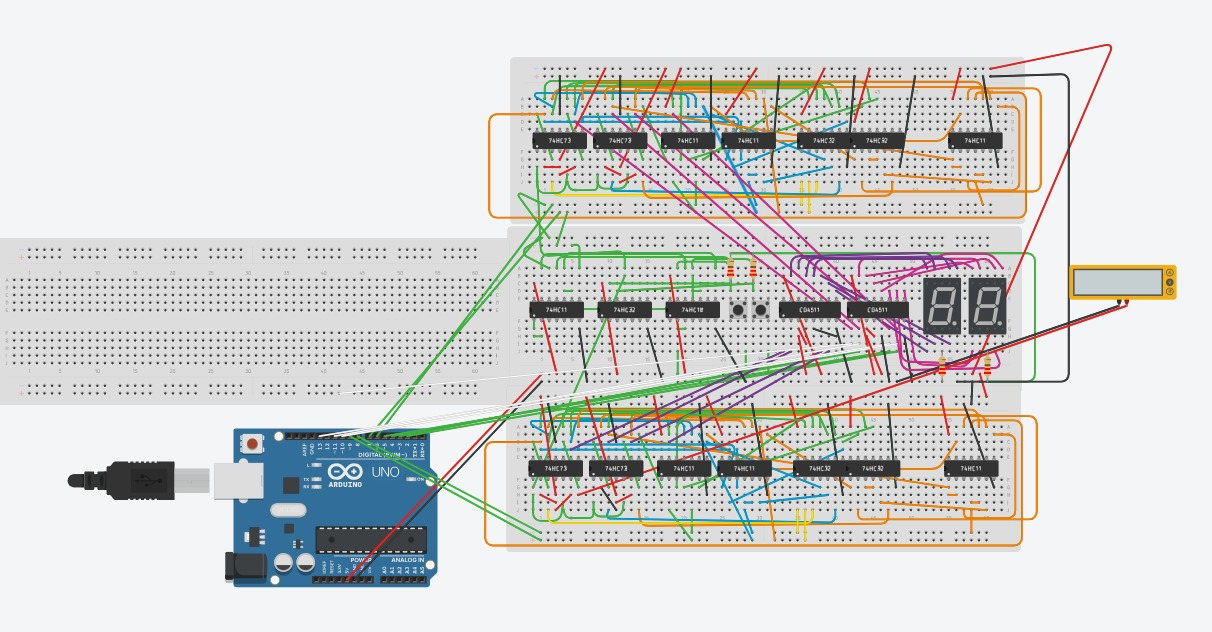
\includegraphics[width=\textwidth]{counter_circuit.jpeg}
        \caption{BCD counter circuit simulation.}
	\label{fig(a):bcd_counter_simulating}
    \end{figure}
    \begin{figure}[H]
	    \centering
	    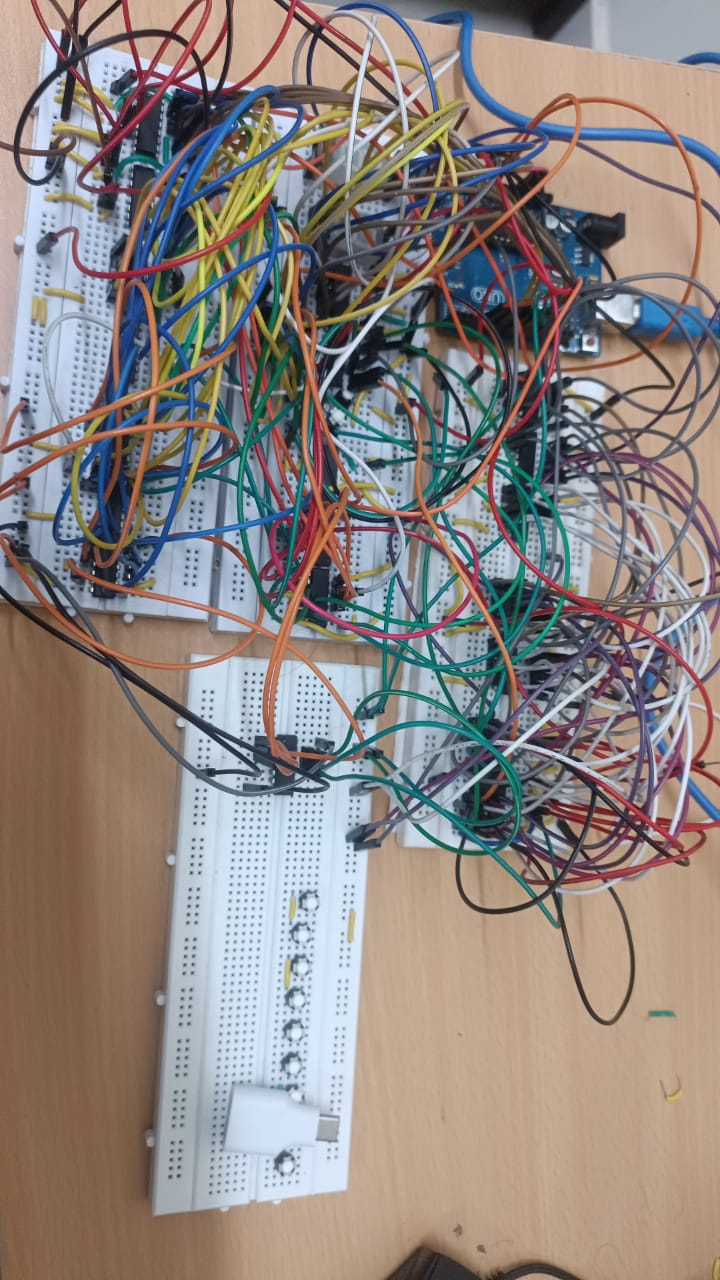
\includegraphics[width=\textwidth]{circuit.jpeg}
	    \caption{BCD counter circuit design}
	    \label{fig(b):BCD_Counter_design}
    \end{figure}
    \newpage
    \subsection{Wiring}
    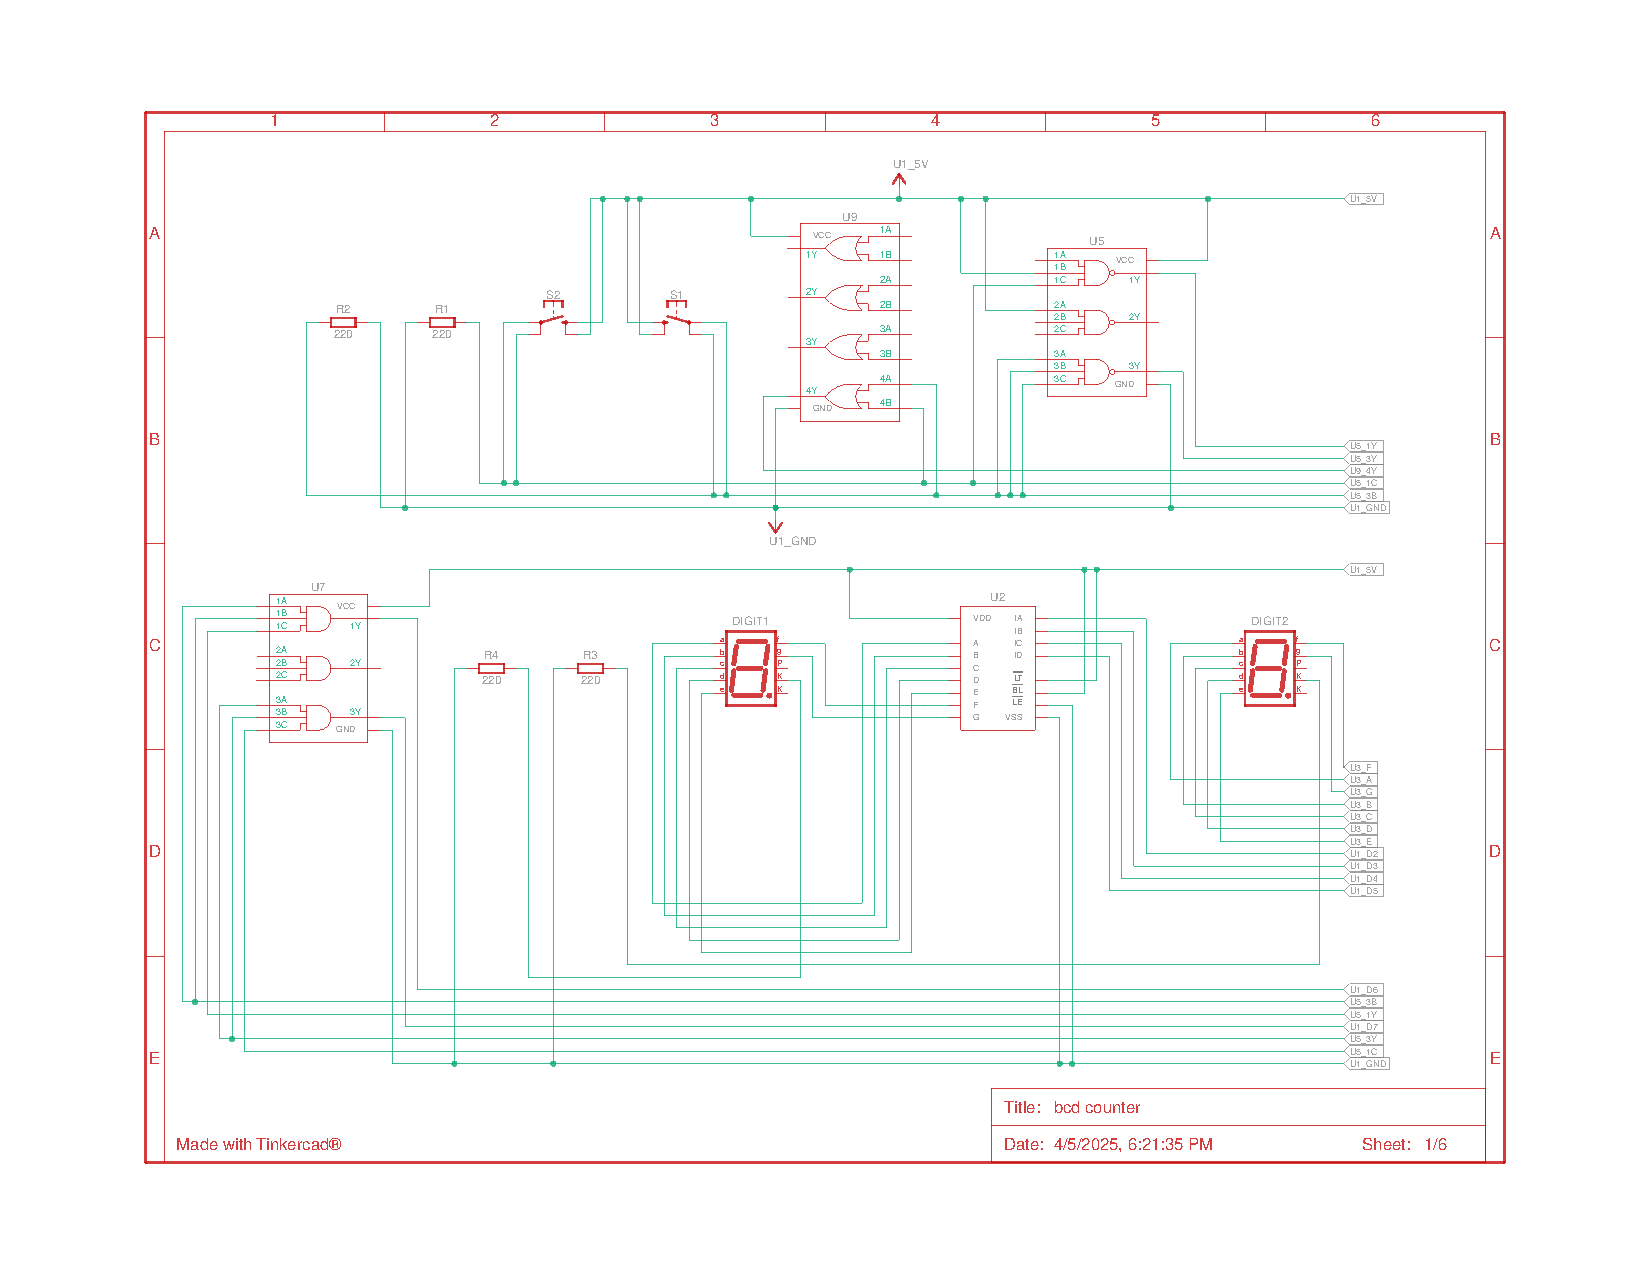
\includepdf[pages=-]{bcd counter.pdf}
    \section{Conclusion}
    The above circuit performs number counting from 0 to 99.When up button is pressed the number increases by one and down button is pressed number decreases by one
    
    To refer arduino code and working video refer to \\
    \url{https://github.com/ArnavYadnopavit/ElectricalLabEE1200/tree/main/Labreport8}\\
    
 \centering
 Thank you
    \end{document}
